\section{Adoption Focused Platforms} \label{chapter3:software-abstraction}

Section \ref{chapter3:software-maintainability} and section \ref{chapter:software-performance} presented the platforms focusing on maintainability and performance efficiency, and showed that focusing on one negatively impacts the other.
A balance between maintainability and performance efficiency is required to have both the community support and the industrial need, required to be widely adopted.
This section presents platforms featuring an abstraction of the tasks organization to propose a compromise between maintainability and performance efficiency.
Section \ref{chap3:software-abstraction:compilers} presents Compilers, and section \ref{chap3:software-abstraction:runtimes} presents Runtime.

% \nt{read and include \cite{Catanzaro2009} it is about Productivity language JIT compilation into efficient language
% And get all the paper that cite this one.}
% \nt{read and include \cite{Engler1994}}
% \nt{read and include \cite{Kovachev2011}}
% \nt{read and include \cite{Asanovic2006}}

\begin{figure}[!h]
\begin{center}
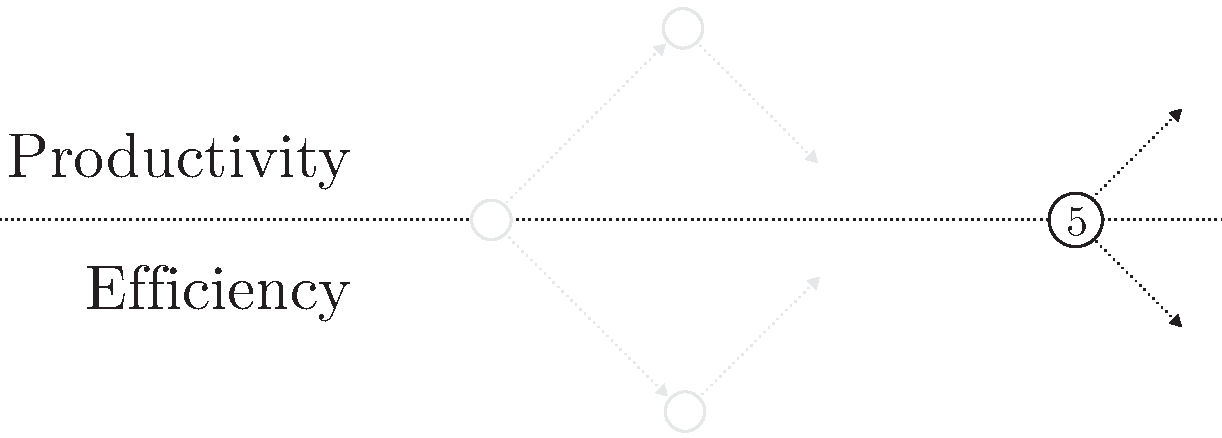
\includegraphics[width=0.6\textwidth]{../ressources/state-of-the-art-5.pdf}
\end{center}
\caption{Focus on Adoption}
\label{fig:state-of-the-art-5}
\end{figure}

\subsection{Abstraction of Tasks Organization}

\subsubsection{Compilers} \label{chapter3:software-abstraction:compilers}

\cit{It is a mistake to attempt high concurrency without help from the compiler}{R. Behren, J. Condit, E. Brewer \cite{Behren2003}}.

As soon as the incompatibility between the modules and the tasks organizations were presented, it was suggested to use a compilation approach to mitigate this incompatibility \cite{Parnas1972}.
% When showing the incompatibility between the two organization, D. Parnas  advocated conciliating the two methods using an assembler to transform the development organization into the execution organization \cite{Parnas1972}.
This section presents the state of the art to extract parallelization from sequential programs through code transformation and compilation.

\nt{read and include \cite{Catanzaro2009}}

\paragraph{Parallelism Extraction}

Extracting parallelism from a sequential implementation is a hard problem \cite{Johnston2004a}.
A compiler needs to identify the commutative operations to parallelize their executions \cite{Rinard1996,Clements2013a}.

An important work was done to parallelize loop iterations \cite{Mauras1989,Amarasinghe1995,Chen2008,Banerjee2013,Radoi2014}, particularly using the polyhedral compilation method \cite{Yuki2013,Grosser2011,Trifunovic2010,Bastoul2004}.
To improve performance gains further, some compilers identify the data-flow inside sequential programs to allow parallelism on the whole program, and not only on its loops \cite{Beck1991,Catanzaro2009,Li2012}.
Moreover, the data-flow representation and execution of a program is well suited for modern data processing applications \cite{Fernandez2014a}, as well as web services \cite{Salmito2013}.
% \nt{TODO Extract parallelism compilers from these :
% Load balanced pipeline parallelism \cite{Kamruzzaman2013}, 
% Regent \cite{Slaughter2015},
% Cilk-P, On-the-Fly Pipeline Parallelism\cite{Lee2013}
% }

% However, the limitation of modular programming regarding parallelization persists.
% In a purely functional language with immutability, higher-order functions are referentially transparent which implies commutativity hence parallelism \nt{Add reference of parallel purely functional languages}.
% \cite{Herrmann2000}
Mutable closures required for higher-order programming remains a challenge to parallelize because of the memory references shared across the program \cite{Harrison1989, Nicolay2010, Matsakis2012a}.
The next paragraphs present some improvements in parallel compilation.
% The first paragraph presents static analysis, while the second presents annotations systems.

% - Continuation-passing style parallelization compilation \cite{Harrison1989}.The interprocedural analysis and automatic parallelization of Scheme programs
% - Automatic Parallelization of Scheme Programs using Static Analysis \cite{Nicolay2010}

% - Commutativity analysis: A new analysis framework for parallelizing compilers \cite{Rinard1996}
% In this paper, they analyze commutative operations to parallelize them.
% It is novel because it isn't about parallelizing loops.
% However, it is not exactly pipeline parallelism either.

% Introducing 'Bones': a parallelizing source-to-source compiler based on algorithmic skeletons \cite{Nugteren2012}

\paragraph{Static analysis}

Compilers statically analyze the control-flow of a program to detect commutative operations \cite{Allen1970}.
The point-to analysis is a popular approach to identify side-effects \cite{Andersen1994,Jang2009,Sridharan2012,Wei2014}.
However, this analysis is not sufficient to track the dynamic control-flow of higher-order functions \cite{Shivers1991} like used in Javascript.

Another approach is the abstract interpretation of the program.
Abstract interpretation techniques are more adapted for dynamic languages like Javascript, and are successfully used for security applications \cite{Huang2004,Jovanovic2006,Yu2007,Maffeis2009a,Chudnov2015,Dolby2015}\nt{Update the citation for Dolby2015}.
It allows to statically reason on the behavior of dynamic program \cite{Maffeis2008,Smith2011,Gardner2012,Hackett2012,Raychev2013,Gardner2013,Bodin2014}.

However, static analysis techniques are too imprecise, and expensive for the performance gain to be profitable.
Instead, some compilers relies on annotations from the developers.

\paragraph{Annotations}

Some works proposed to rely on annotations from the developer to identify the commutativity of operations or the shared data structures \cite{Vandierendonck2010a,Fernandez2014a}.
Such annotations are especially relevant for accelerators such as GPUs or FPGAs, because the development effort yield huge performance improvements \cite{Tarditi2006}.
Examples of such compilers are OpenMP \cite{Dagum1998}, OpenCL \cite{Stone2010}, CUDA \cite{Nvidia2007} Cg \cite{Mark2003}, Brook \cite{Buck2004}, Liquid Metal \cite{Huang2008}.

% Bloom declarative language \ftnt{http://bloom-lang.net/}
% Blazes: Coordination analysis for distributed programs \cite{Alvaro2014}

% Livescript
% Typescript 
% Annotations, but not for parallelism.
% Asynchronism annotations should be sufficient.

\paragraph{Compilation Limitations}

The static analysis of static, low level languages like FORTRAN or C, brings performance improvements.
However for more dynamic, higher-level languages like Javascript, the static analysis is not sufficient to identify correctly the dependencies between operations to parallelize them.
And parallel compilers often fall back on relying on annotation provided by developers.
Hence, the burden of detecting commutativity of operations falls back to the developer, similarly to the platforms presented in the section \ref{chapter3:software-performance}, focusing on performance efficiency.

Alternatively, another approach is to dynamically distribute the commutative operations, and assure the communications.
The next paragraphs present runtime allowing this dynamic distribution.

\subsubsection{Runtimes} \label{chapter3:software-abstraction:runtimes}

\paragraph{Partitioned Global Address Space}

The Partitioned Global Address Space (PGAS) provides the developers with a uniform memory access on a distributed architecture.
It attempts to combine the performance efficiency of distributed memory systems, with the maintainability of shared memory systems.
Each computing node executes the same program, and provide its local memory to be shared with all the other nodes.
The PGAS platform assures the remote accesses and synchronization of memory across nodes.
Examples of implementation of the PGAS model are 
CoArray Fortran \cite{Numrich1998},
X10 \cite{Charles2005}.
Unified Parallel C \cite{El-Ghazawi2006},
Chapel\cite{Chamberlain2007},
OpenSHMEM \cite{Chapman2010}.
Kokko \cite{Edwards2012},
UPC++ \cite{Zheng2014},
RAJA \cite{Hornung2014},
ACPdl \cite{Ajima2015} and
HPX \cite{Kaiser2014,Kaiser2015}


\paragraph{Dynamic Distribution of Execution}

An interesting work following SEDA, is Leda \cite{Salmito2013,Salmito2014}.
% It follows the PCAM design methodology \cite{Foster1995} to 
It proposes a model where the stages of the pipeline are defined only by their role in the application.
% Partition $\to$ Communicate $\to$ Agglomerate $\to$ Map.
The actual execution distribution is defined automatically during deployment. % , only after the development
% blurs the distinction between the parallel organization of execution, and the modular organization of implementation.
This automation manages the execution organizations to help the developer focus on the modular organization.




\paragraph{}

Tables \ref{tab:abstraction-maintainability} and \ref{tab:abstraction-performance} presents the platforms presented in this section regarding maintainability and performance.

\AbstractionMaintainabilityTable{tab:abstraction-maintainability}

\AbstractionPerformanceTable{tab:abstraction-performance}



\subsection{Adoption Limitations}

All the platforms presented in this section come from the need to reduce the development commitment required for performance efficiency.
However, none of these platforms are highly supported by the community because they respond exclusively to industrial needs.

They are limited to scientific applications.

The balance between performance efficiency and maintainability is not sufficient for a community of passionate to gather around the platform.
The platform needs to allow the community to experiment and to start projects.
The context of web development is particularly suited to experiment and start projects.

\AbstractionAdoptionTable{tab:abstraction-performance}

\subsection{Summary}

Table \ref{tab:abstraction-summary} summarizes the characteristics of the platforms presented in this section.

\AbstractionSummaryTable{tab:abstraction-summary}

\endinput
























\section{Due Related works} \label{section:related}

To our knowledge, our work is the first to explore the transformation from continuations to Promises in Javascript, and to state the similarity between Promises and data-flow programming.
This section presents the various works related to ours.
Our work is based on the previous work on Promises and Futures~\cite{Liskov1988}, and their specifications in Javascript\footnote{\url{https://promisesaplus.com/}}\footnote{\url{https://people.mozilla.org/~jorendorff/es6-draft.html\#sec-promise-objects}}.


Because of its dominant position in the web, Javascript is recently subject to a growing interest in the field of static analysis.
We identify two teams working on static analysis for Javascript.
In the Department of Computing, Imperial College London, S. Maffeis, P. Gardner and G. Smith realised a large body of work around the static analysis of Javascript.
Their work is based around an operational semantic~\cite{Maffeis2008} to bring program understanding~\cite{Smith2011,Gardner2012,Gardner2013,Bodin2014}.
Their goal seems to revolve around security applications of this analysis~\cite{Maffeis2009,Maffeis2009a}.
In a collaboration between the programming language research groups at Aarhus University and Universität Freiburg, P. Thiemann, S. Jensen and A. Møller are working on the static analysis of Javascript.
They presented a tool providing type inference using abstract interpretation~\cite{Thiemann2005,Jensen2009,Jensen2012}.
Their goal is to improve the tools available for Javascript developers~\cite{Andreasen}.
Another example of interest for Javascript static analysis is the adaptation of the points-to analysis from L. Andersen's thesis~\cite{Andersen1994} to Javascript, by D. Jang \textit{et al.}~\cite{Jang2009} and S. Wei \textit{et al.}~\cite{Wei2014}.

The industry seems to follow the same trends.
There are some security tools based on static analysis.
We can cite for example, the company Shape Security\footnote{\url{https://shapesecurity.com/}}.
They developed \textit{Esprima}, a Javascript parser, and a serie of tools to help static analysis.
Facebook released flow\footnote{\url{http://flowtype.org/}} on 26 October 2014, a static type checker for Javascript.

Promises combine controls over the execution and the data flow.
It arrange the execution parts sequentialy and assign the result of one into the inputs of the next.
This arrangement seems similar to some works on the field of functional and data-flow programming~\cite{Johnston2004,Cohen2012,Morrison1994,Kahn1974}.
We consider it a first step in the merge of elements from the data-flow paradigm into the imperative paradigm.
The Functional Reactive Programming paradigm pushes the intrication of data and control-flow even further~\cite{Winograd-Cort2013}.
